\begin{figure}
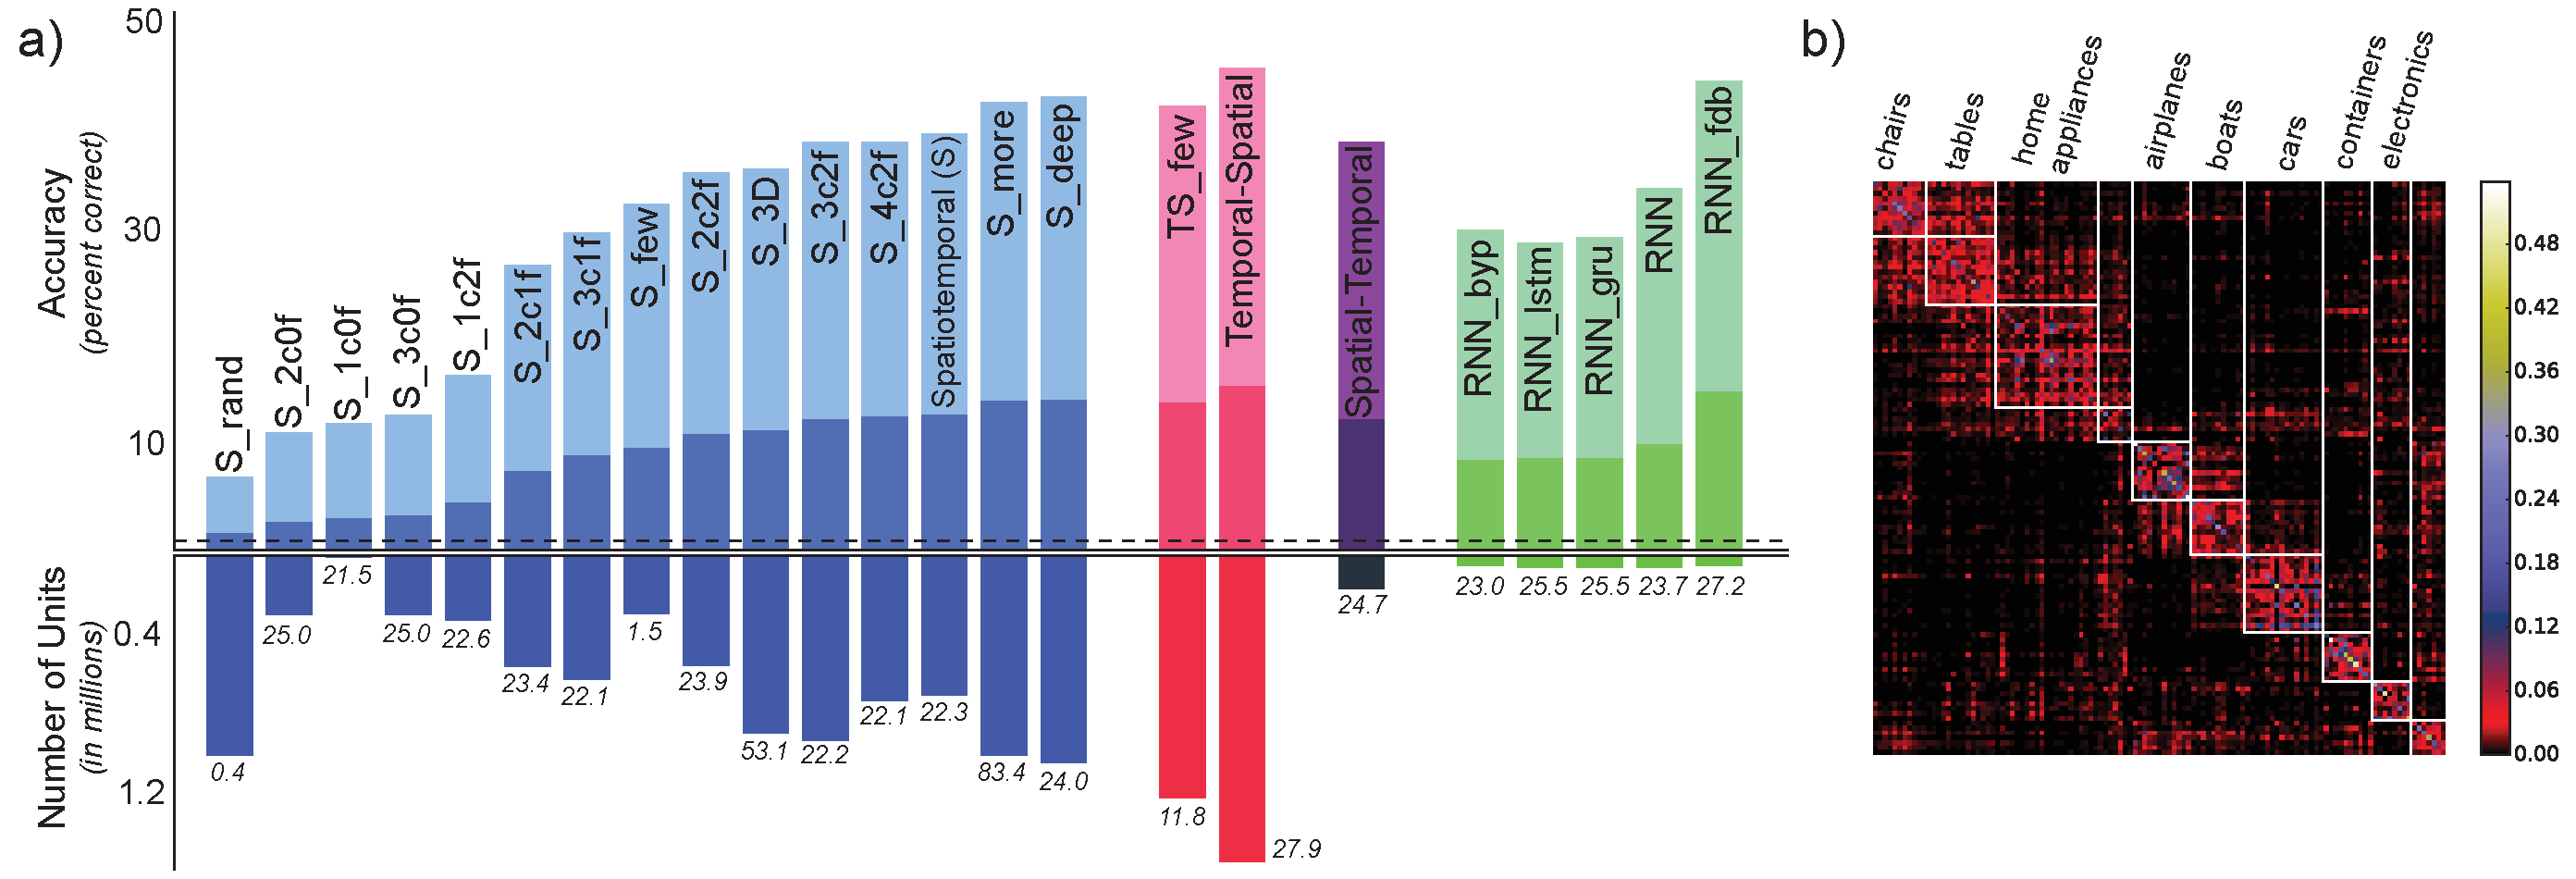
\includegraphics [width=1\linewidth]{figures/results.pdf}
\vspace{-2mm}
\caption{\textbf{Performance results.} \textbf{a.} Each bar in this figure represents one model. The positive $y$-axis is performance measured in percent correct (top1=dark bar, chance=0.85\%, top5=light bar, chance=4.2\%).   The negative $y$-axis indicates the number of units in networks, in millions of units.  Model architecture family is indicated by color.  The definition of individual model labels can be found in the Results section. \textbf{b.} Confusion Matrix for the highest-performing model (in the Temporal-Spatial family).~\label{fig_main}}
\end{figure}

\textbf{Model Performance:} 
Our strategy in identifying potential models of the whisker-trigeminal system is to explore many specific architectures within each architecture family, evaluating each specific architecture both in terms of its ability to solve the shape recognition task in our training dataset, and its efficiency (e.g. number of parameters and number of overall units).
Because it can be misleading to compare models with different numbers of parameters, we generally evaluated models with similar numbers of parameters: exceptions are noted where they occur.
As we evaluated many individual structures within each family, a list of the specific models and parameters are given in the supplementary materials.

Our results (Fig. \ref{fig_main}) can be summarized with following conclusions:

\begin{itemize}[leftmargin=*,itemsep=0ex,topsep=1ex]
   \item Many specific network choices within all families do a comparatively poor job at the task, achieving just-above-chance performance.
   \item However, within each family, certain specific choices of parameters lead to much better network performance.
   Overall, the best performance was obtained for the Temporal-Spatial model, with 15.2\% top-1 and 44.8\% top-5 accuracy.
   Visualizing a confusion matrix for this network (Fig. \ref{fig_main})b  and other high-performing networks indicate that the errors they make are generally reasonable.
   \item Training of filters was extremely important for performance; no architecture with random filters performed above chance levels.
   \item Depth of the architecture was a very important factor in performance. Architectures with fewer than four layers achieved substanially lower performance than somewhat deeper ones.
   \item Number of parameters in the model was a somewhat important factor in performance within an architecture family, but only to a point, and not between architectural families.
   The Temporal-Spatial architecture, was able to outperform other classes while using significantly fewer parameters.
   \item Recurrent networks with long-range feedback were able to perform nearly as well as the Temporal-Spatial model with equivalent numbers of parameters, while using far fewer units.
   These long-range feedbacks appeared critical to performance, with purely local recurrent architectures (including LSTM and GRU) achieving significantly worse results.
\end{itemize}

\begin{figure}
%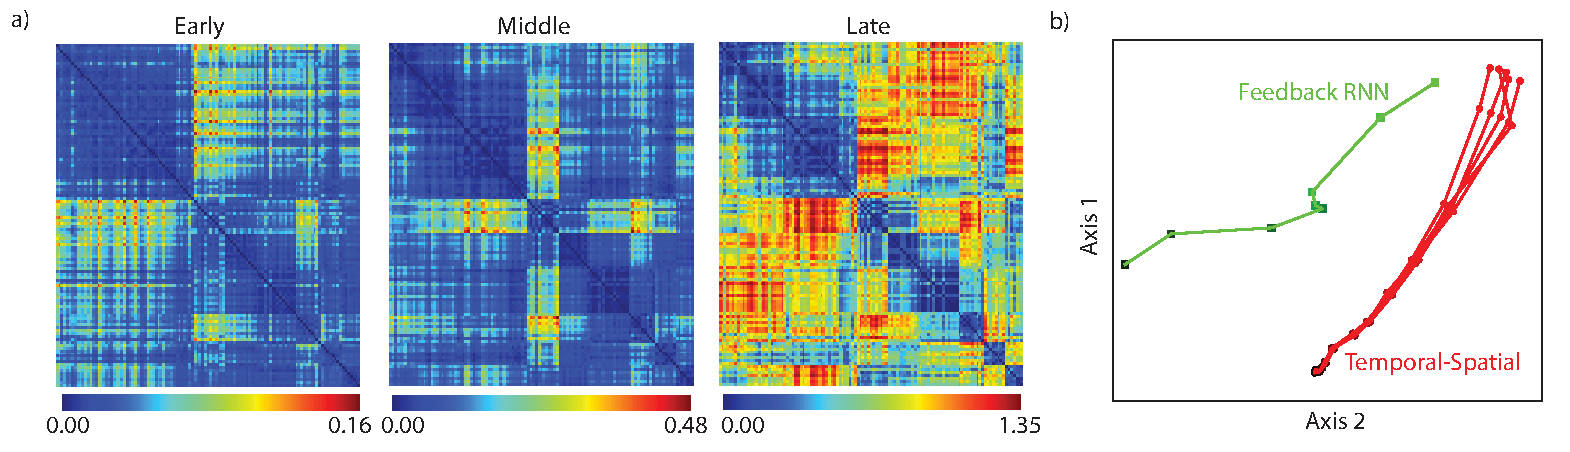
\includegraphics [width=1\linewidth]{figures/rdms.pdf}
\vspace{-2mm}
\caption{\textbf{Using RDMs to Discriminate Between High-Performing Models.} \textbf{a.} Representational Dissimilarity Matrices (RDMs) for selected layers of a high-performing network from Fig. \ref{fig_main}a, showing low, intermediate and higher model layers.  Model feature vectors are averaged over classes in the dataset prior to RDM computation, and RDMs are shown using the same ordering as in Fig. \ref{fig_main}b. \textbf{b.} Two-dimensional embedding of RDMs for several models.   ~\label{fig_rdms}}
\end{figure}

\textbf{Model Discrimination:}  The above results indicated that we had identified several high-performing networks in quite distinct architecture families.
In other words, the strong performance constraint allows us to identify several specific candidate model networks for the biological system, cutting down a much larger set of mostly non-performing neural networks into a kind of ``shortlist''.
Given this result, the key biologically relevant follow-up question is then: how should we distinguish between the elements in the shortlist?
What signatures of the differences between architectures could be extracted from data obtainable experiments that are practically realizable with today's neurophysiological tools?

To help address this question, we used Representational Dissimilarity Matrix (RDM) analysis~\cite{Kriegeskorte2008}.
For a set of stimuli $S$, RDMs are $|S| \times |S|$-shaped correlation distance matrices taken over the feature dimensions of a representation, e.g. matrices with $ij$-th entry $RDM[i, j] = 1 - corr(F[i], F[j])$ for stimuli $i, j$ and corresponding feature output $F[i], F[j]$.
The RDM characterizes the geometry of how a given representation lays out stimuli in a way that is independent of the individual feature dimensions, and can thus be compared effectively between different feature representations of the same data.
RDMs have been useful in establishing connections between deep neural networks and neural data from the ventral visual stream~\cite{cadieu2014deep, Yamins2014, khaligh2014deep}. 
RDMs are readily computable from neural response pattern data samples, and are in general have bene found to be comparatively robust to variability due to experimental randomness (e.g. electrode/voxel sampling).
We obtained RDMs for several of our high-performing models, computing RDMs separately for each model layer (Fig. \ref{fig_rdms}a), averaging feature vectors over different swipes of the same object before computing the correlations.
This lead to $9981\times9981$-sized matrices (since there were 9,981 distinct object in our dataset).
We then computed distances between each layer of each model in this $9981\times9980/2$-dimensional RDM space.
To determine if differences in this space between models and/or layers were significant, we computed RDMs for multiple instances of each model trained with different initial conditions, and compared the between-model to within-model distances.
We found that while the top layers of models were similar (likely owing to the fact that they were all trained on the same task), intermediate layers diverged substantially between models, by amount that was larger than both the initial-condition-induced variability within a model layer and between different layers of the same model (Fig. \ref{fig_rdms}b).
This result is not surprising, given the fact that the models are quite structurally different, but its utility is that it strongly suggests that a conceptually simple and potentially feasible neuroscience experiment could distinguish between them: namely, measuring batteries of neural responses in several areas of the whisker trigeminal system, computing the RDMs from these data, and then comparing to those of the models. 



